\chapter{The data}
\begin{figure}[H]
	\centering
	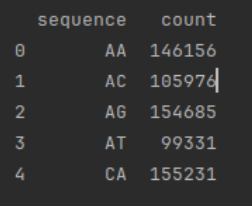
\includegraphics[width=0.7\linewidth]{../figures/data_example}
	\caption{An example of the data}
	\label{fig:data0}
\end{figure}

In the first column we have the k-mer, in this specific figure it is a 2-mer, and in the second column we have the count of that specific sequence. In addition to the control and the test samples, we also have a background file, which details the total number of combinations of sequences.
